%!TEX TS-program = xelatex
\documentclass[]{friggeri-cv}
\usepackage{graphicx}
\addbibresource{bibliography.bib}

\begin{document}
\header{Olivier }{Gayot}
       {Etudiant en 3ème année}


% In the aside, each new line forces a line break
\begin{aside}
    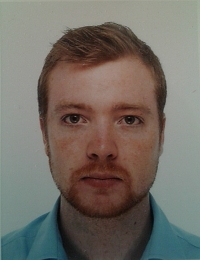
\includegraphics[width=100pt]{photo.png}
  \section{A propos}
    26 rue Saint Dizier
    54000 Nancy
    --
    21 ans
    Permis B
    --
    ~
    téléphone: +33663613699
    \href{mailto:ogayot@free.fr}{ogayot@free.fr}
    \href{https://github.com/duskCoder}{github: duskCoder}
    \href{http://www.sigexec.com}{http://www.sigexec.com}
  \section{langues}
    français: langue maternelle
    anglais: courant
\end{aside}

\section{Centres d'intéret}

Développement bas niveau\\
Sécurité informatique (exploitation et prévention)\\
Développement embarqué\\
Découverte de nouvelles technologies

\section{Education}

\begin{entrylist}
  \entry
    {depuis 2011}
    {formation de 5 ans en développement informatique}
    {EPITECH Nancy}
    {}
  \entry
    {2011}
    {Baccalauréat Scientifique avec mention}
    {Lycée Raymond Poincaré, Bar le Duc}
    {Spécialité Sciences de l'Ingénieur}
\end{entrylist}

\section{Expérience}

\begin{entrylist}
  \entry
    {depuis 2013}
    {Fun RC Toys, Messein}
    {Partenariat pour un projet d'étude}
    {\emph{Développement d'un module de sécurité pour les drones (surtout quadricoptères) avec trois autres étudiants}}
  \entry
    {depuis 2013}
    {Intersec, Paris}
    {Développeur en alternance}
    {\emph{Amélioration du logiciel développé pendant mon stage (voir ci dessous)}}
  \entry
    {sept. -> dec. 2012}
    {Intersec, Paris}
    {Stage au sein de l'équipe de Recherche et développement}
    {\emph{Développement d'un logiciel capable de simuler les mouvements d'un large réseau d'abonnés qui se déplacent intelligement à l'intérieur d'une zone donnée}}
\end{entrylist}

\section{Technologies}
\begin{entrylist}
  \entry
    {C}
    {Expérimenté}
    {}
    {Usage intensif du standard C99 et des extensions GNU}
  \entry
    {C++}
    {Intermédiaire}
    {}
    {Assez bonnes notions du paradigme object}
  \entry
    {Assembleur}
    {Intermédiaire}
    {}
    {Jeux d'instructions IA-32 et x86\_64\\
    Ecriture et rétro ingénierie}
  \entry
    {Web}
    {Connaissances des technologies web courantes}
    {}
    {XHTML/CSS\\
        Scripting côté serveur: PHP\\
        Scripting côté client: JavaScript (+ jQuery)
    }
  \entry
    {Python 2\&3}
    {Débutant}
    {}
    {J'écris actuellement un wrapper pour la libelf afin d'en apprendre plus sur le langage}
  \entry
    {Perl}
    {Débutant}
    {}
    {}
\end{entrylist}
\section{Logiciel}
\begin{entrylist}
  \entry
    {}
    {Usage journalier de GNU/Linux et occasionnel de Microsoft Windows}
    {}
    {Utilisation intensive de Vim\\
    (D)CVS: Git, Subversion\\
    GNU Autotools, make, GCC\\
    Débogage: gdb, valgrind, ollydbg}

\end{entrylist}

\section{Divers}
\begin{entrylist}
  \entry
    {}
    {}
    {}
    {Connaissance du format ELF\\
    Membre actif de l'ASEN (\emph{Association de Sécurité d'EPITECH Nancy})\\
    Solides connaissances des avantages et inconvéniants liés à l'utilisation des langages dits "unsafe"}
\end{entrylist}

\end{document}
